\documentclass{article}
\usepackage[utf8]{inputenc}
\usepackage{geometry}
\usepackage{tikz}

\usepackage{graphicx}
\graphicspath{{images/}}

\usepackage{float}
\usepackage{caption}
\usepackage{subcaption}
\captionsetup{compatibility=false}

\usepackage{hyperref}
\hypersetup{
  colorlinks,
  citecolor=black,
  filecolor=black,
  linkcolor=black,
  urlcolor=blue
}

\title{Polytope}
\author{URL, Mathtician, }
\date{February 2021}

\begin{document}

\maketitle

\section{Introduction}
Welcome to the \href{https://discord.gg/invite/zMRu7T4}{Polytope Discord}!

\section{What is a polytope?}
A \textbf{polytope} is a general name for
\textbf{polygons} (2D), \textbf{polyhedra} (3D), \textbf{polychora} (4D),
and so on for any dimension.
As with many terms used on the Polytope Discord,
the word ``polytope'' can have a few definitions which are not completely equivalent.
All of the commonly-used ones, however, agree on the following:
\begin{itemize}
\item
  A polytope in $n$ dimensions (known hereafter as an $n$-polytope)
  is made of \textbf{facets} which are $(n-1)$-polytopes.
  \begin{itemize}
  \item Polychora ($4$-polytopes) have facets which are polyhedra ($3$-polytopes),
  \item whose facets are polygons ($2$-polytopes),
  \item whose facets are line segments ($1$-polytopes),
  \item whose facets are points ($0$-polytopes)!
  \end{itemize}
\item
  More stuff here, although the next section might break up the list,
  so it might be good not to format the whole def in terms of a list
  so that we can fit in more explanations.
\end{itemize}

For example, consider the following triangle $\Delta$ABC.

\begin{center}
  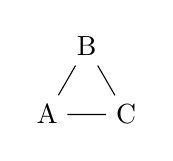
\begin{tikzpicture}
    \node (a) at (0,0) {A};
    \node (b) at (0.5,0.866) {B};
    \node (c) at (1,0) {C};
    \draw (a) -- (b) -- (c) -- (a);
  \end{tikzpicture}
\end{center}

It is a polygon which contains three line segments,
or \textbf{edges}, as they are known
when mentioned as part of a larger polytope.
It also contains three points, or \textbf{vertices},
or even \textbf{verts} for short.
(In the polytope world, abbreviations are everywhere!)
More specifically, its facets are the edges
$\overline{\rm AB}$, $\overline{\rm AC}$, and $\overline{\rm BC}$,
and their facets are the vertices A, B, and C.
We keep track of what has what as a facet using a \textbf{Hasse diagram},
which is shown below for $\Delta$ABC.

\begin{center}
  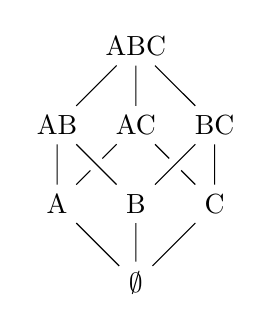
\begin{tikzpicture}
    \node (abc) at (0,2) {ABC};
    \node (ab) at (-1,1) {AB};
    \node (ac) at (0,1) {AC};
    \node (bc) at (1,1) {BC};
    \node (a) at (-1,0) {A};
    \node (b) at (0,0) {B};
    \node (c) at (1,0) {C};
    \node (o) at (0,-1) {$\emptyset$};
    \draw (o) -- (a) -- (ab) -- (abc) -- (ac) -- (c)
    (b) -- (o) -- (c) -- (bc) -- (abc)
    (a) -- (ac);
    \draw[preaction={draw=white, -,line width=6pt}] (ab) -- (b) -- (bc);
  \end{tikzpicture}
\end{center}

\section{Regular polytopes}
There are multiple definitions for when a polytope is \textbf{regular},
but they all require every element (vertices, edges, faces, etc.) to ``look the same.''

\section{Uniform polytopes}
General polytopes can be very complicated. Therefore, we only tend to study specific categories of polytopes. The type of polytopes we study most in this server are \textbf{uniform polytopes}.

Uniformity is defined recursively. In 2D, uniform polytopes are simply the regular polygons.
In higher dimensions, uniform polytopes are those whose facets are all uniform. To see what we mean, let's look at a few examples.

\begin{figure}[H]
  \centering
  \begin{subfigure}{.33333\textwidth}
    \centering
    \includegraphics[width=.5\linewidth]{tut}
    \caption{Truncated tetrahedron}
    \label{fig:tut}
  \end{subfigure}%
  \begin{subfigure}{.33333\textwidth}
    \centering
    \includegraphics[width=.5\linewidth]{did}
    \caption{Dodecadodecahedron}
    \label{fig:did}
  \end{subfigure}%
  \begin{subfigure}{.33333\textwidth}
    \centering
    \includegraphics[width=.5\linewidth]{snid}
    \caption{Snub icosidodecahedron}
    \label{fig:snid}
  \end{subfigure}%
  \caption{Three examples of uniform polyhedra.}
  \label{fig:uniforms3D}
\end{figure}

In 3D, the uniform polytopes have already been enumerated. It turns out that, aside from the infinite families of \textbf{prisms} and \textbf{antiprisms}, there's exactly 75 uniform polyhedra.

\begin{figure}[H]
  \centering
  \begin{subfigure}{.5\textwidth}
    \centering
    \includegraphics[width=.5\linewidth]{hep}
    \caption{Heptagonal prism}
    \label{fig:hep}
  \end{subfigure}%
  \begin{subfigure}{.5\textwidth}
    \centering
    \includegraphics[width=.5\linewidth]{heap}
    \caption{Heptagonal antiprism}
    \label{fig:heap}
  \end{subfigure}%
  \caption{An example of a prism and an antiprism. These can be built from any regular polygon, and made uniform in all cases.}
  \label{fig:prisms}
\end{figure}

In 4D and higher up, the problem remains unsolved. In 4D, we know of two infinte families and 2194 uniform polychora. In 5D and up, we haven't yet done a thorough examination, though we know of various families of uniforms such as \textbf{Wythoffians} (those generated by a Coxeter diagram), and \textbf{multiprisms}.

\section{CRF polytopes}
A polytope is called \textbf{convex regular-faced}, or \textbf{CRF} for short, when it is convex (without dents, holes or self-intersections) and all of its faces are regular. Let's look at a few examples.

\begin{figure}[h]
  \centering
  \begin{subfigure}{.33333\textwidth}
    \centering
    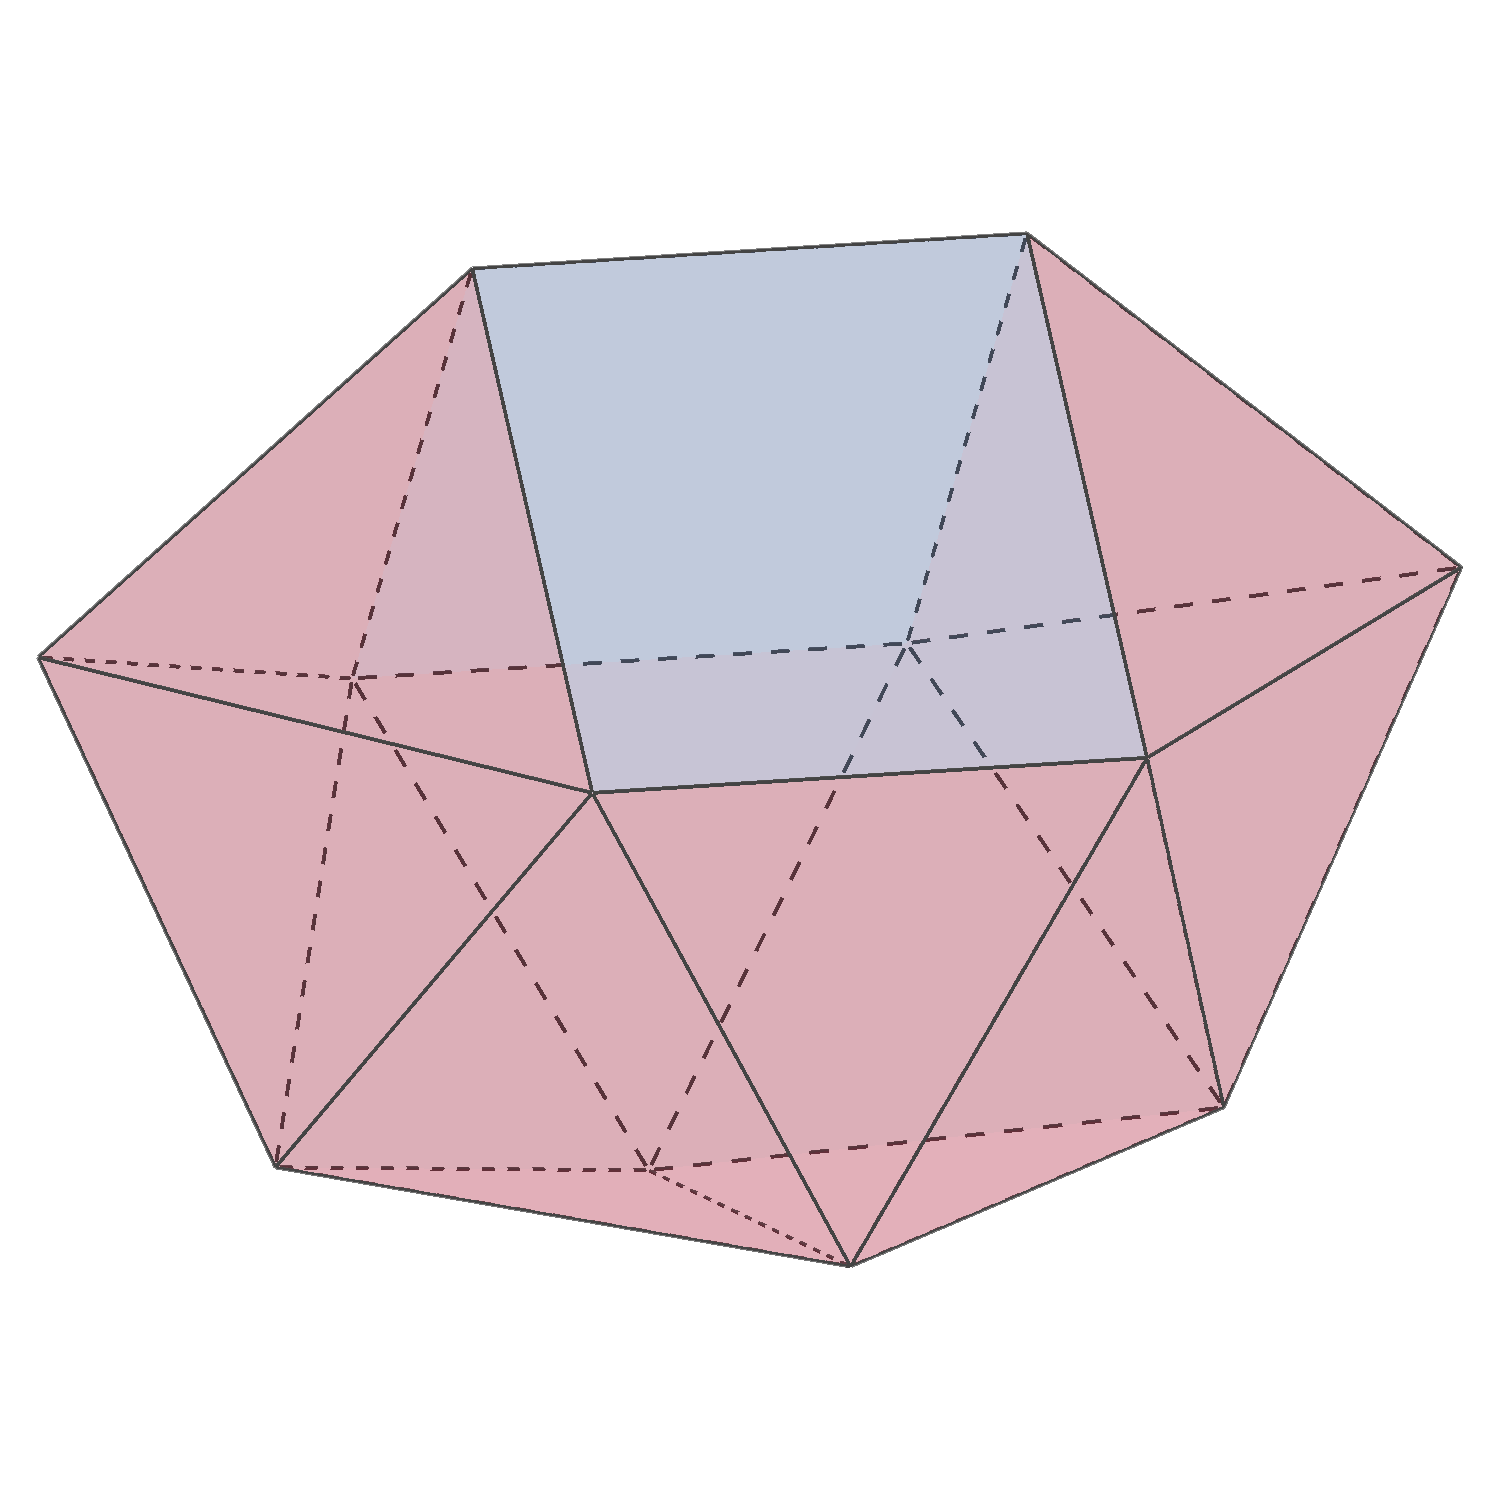
\includegraphics[width=.5\linewidth]{Sphenomegacorona}
    \caption{Sphenomegacorona}
    \label{fig:polyhedra_1}
  \end{subfigure}%
  \begin{subfigure}{.33333\textwidth}
    \centering
    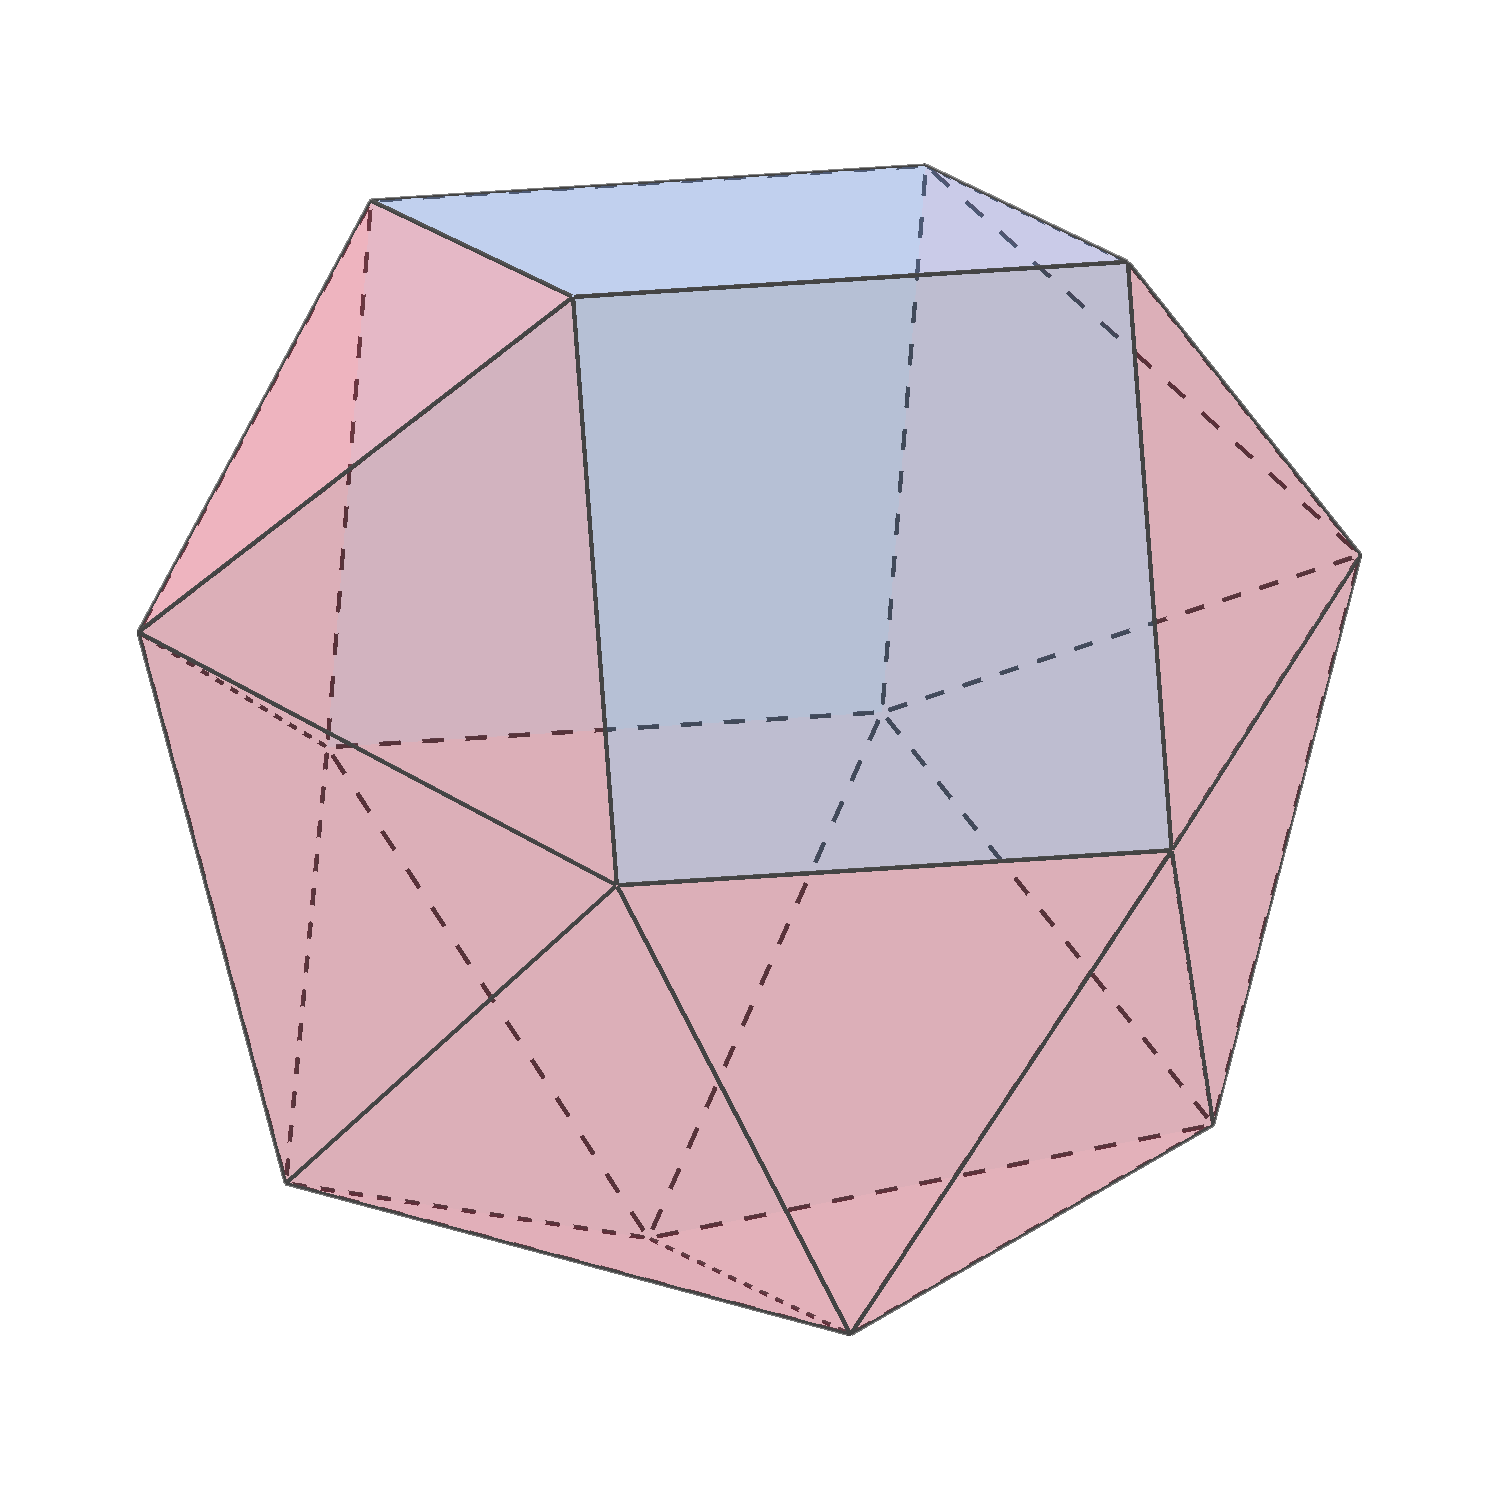
\includegraphics[width=.5\linewidth]{Hebesphenomegacorona}
    \caption{Hebesphenomegacorona}
    \label{fig:polyhedra_2}
  \end{subfigure}%
  \begin{subfigure}{.33333\textwidth}
    \centering
    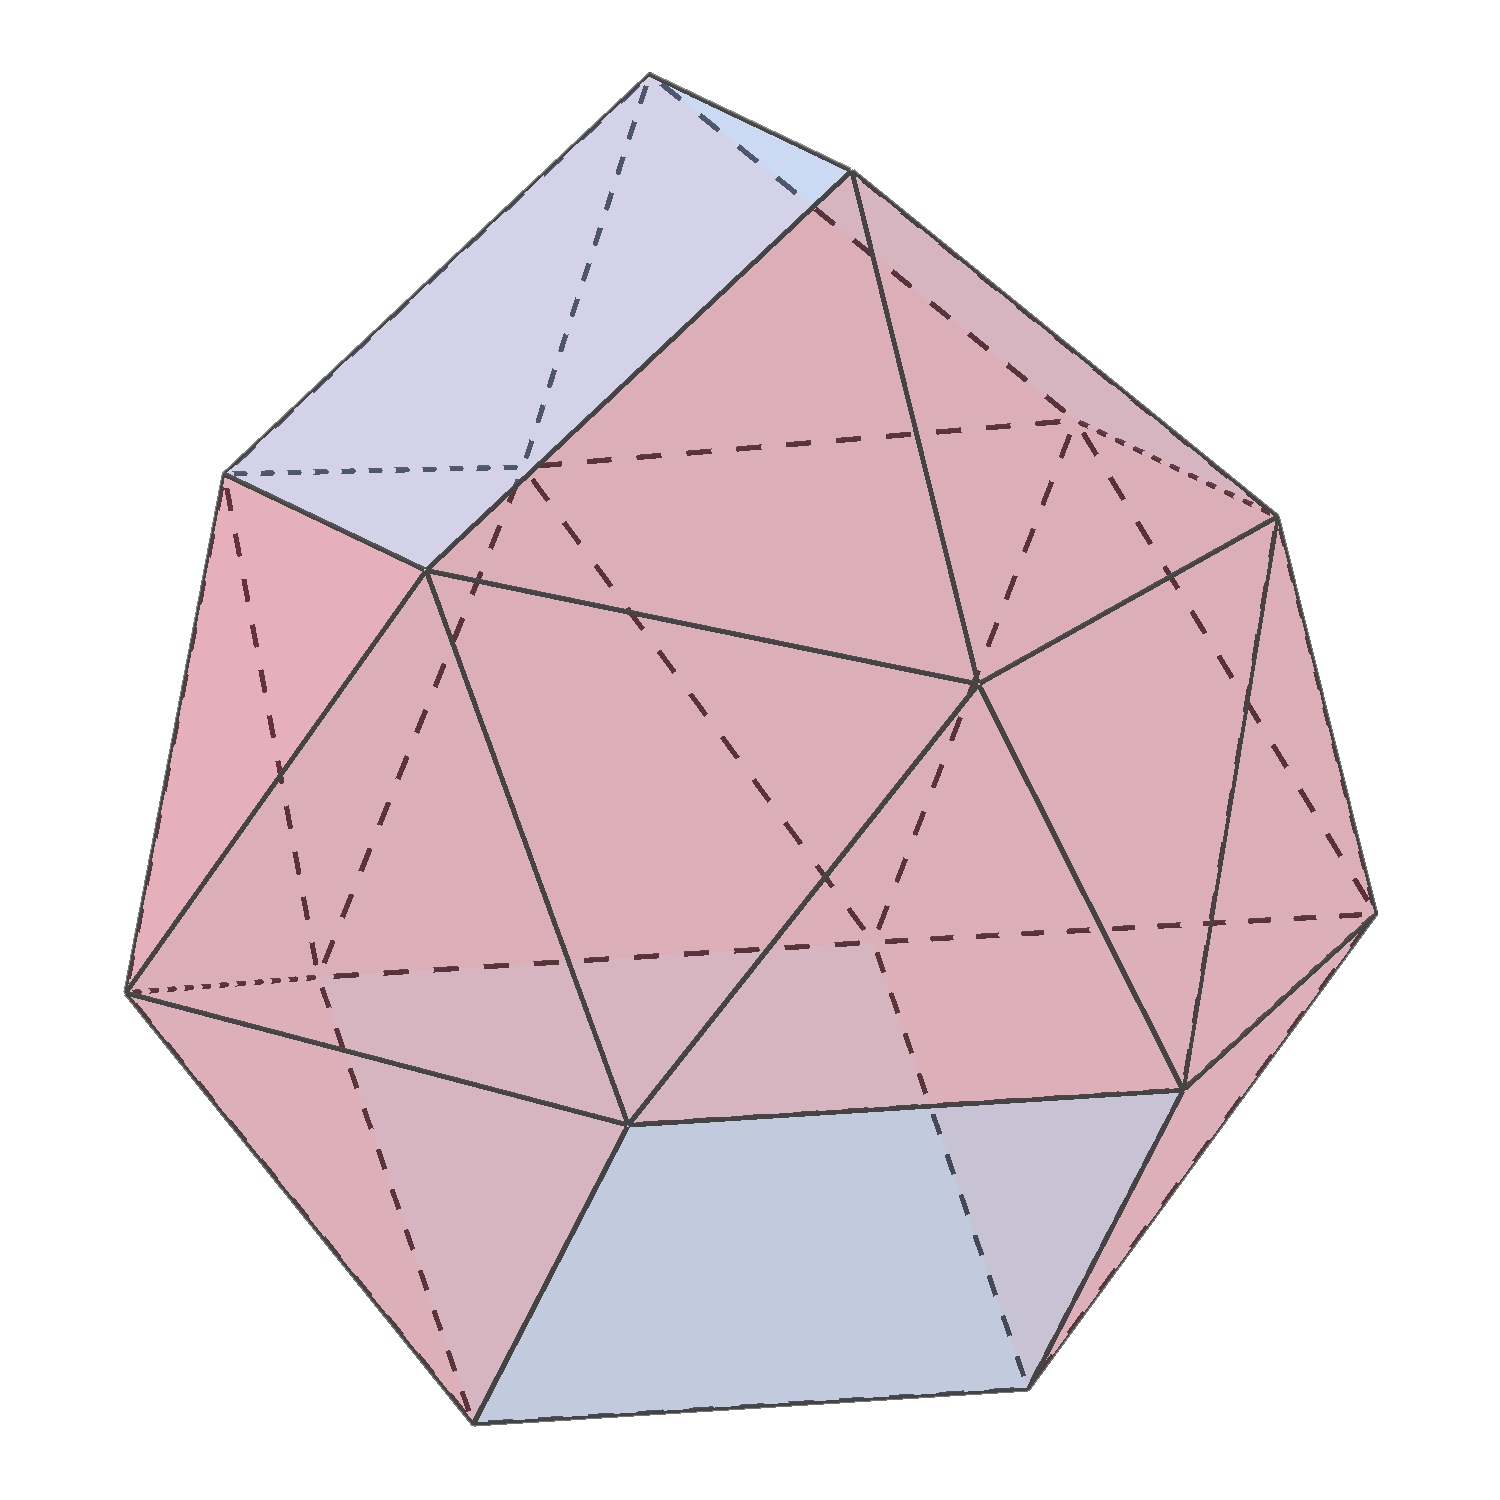
\includegraphics[width=.5\linewidth]{Disphenocingulum}
    \caption{Disphenocingulum}
    \label{fig:polyhedra_3}
  \end{subfigure}%
  \caption{Test images!}
  \label{fig:polyhedra}
\end{figure}


\end{document}
